% Copyright 2006 by Till Tantau
%
% This file may be distributed and/or modified
%
% 1. under the LaTeX Project Public License and/or
% 2. under the GNU Free Documentation License.
%
% See the file doc/generic/pgf/licenses/LICENSE for more details.


\section{Transparency}

\label{section-tikz-transparency}


\subsection{Overview}

Normally, when you paint something using any of \tikzname's commands
(this includes stroking, filling, shading, patterns, and images), the
newly painted objects totally obscure whatever was painted earlier in
the same area.

You can change this behaviour by using something that can be thought
of as ``(semi)transparent colors.'' Such colors do not completely
obscure the background, rather they blend the background with the new
color. At first sight, using such semitransparent colors might seem quite
straightforward, but the math going on in the background is quite
involved and the correct handling of transparency fills some 64 pages
in the PDF specification. 

In the present section, we start with the different ways of specifying
``how transparent'' newly drawn objects should be. The simplest way is
to just specify a percentage like ``60\% transparent.'' A much more
general way is to use something that I call a \emph{fading,} also
known as a soft mask or a mask.

At the end of the section we adress the problem of creating so-called
\emph{transparency groups}. This problem arises when you paint over a
position several times with a semitransparent color. Sometimes you
want the effect to accumulate, sometimes you do not.

\emph{Note:} Transparency is best supported by the pdf\TeX\
driver. The \textsc{svg} driver also has some support. For PostScript
output, opacity is rendered correctly only with the most recent
versions of GhostScript. Printers and other programs will typically
ignore the opacity setting. 


%Document |fade|, |fading|, |transparency group|, |fading angle|,
%|scope fading| and |scope fading bounding box|.


\subsection{Specifying a Uniform Opacity}

Specifying a stroke and/or fill opacity is quite easy using the
following options.


\begin{key}{/tikz/draw opacity=\meta{value}}
  This option sets ``how transparent'' lines should be. A value of |1|
  means ``fully opaque'' or ``not transparent at all,'' a value of |0|
  means ``fully transparent'' or ``invisible.'' A value of |0.5|
  yields lines that are semitransparent.

  Note that when you use PostScript as your output format,
  this option works only with recent versions of GhostScript.
   
\begin{codeexample}[]
\begin{tikzpicture}[line width=1ex]
  \draw (0,0) -- (3,1);
  \filldraw [fill=examplefill,draw opacity=0.5] (1,0) rectangle (2,1);
\end{tikzpicture}
\end{codeexample}
\end{key}

Note that the |draw opacity| options only sets the opacity of drawn
lines. The opacity of fillings is set using the option
|fill opacity| (documented in Section~\ref{section-fill-opacity}. The
option |opacity| sets both at the same time. 

\begin{key}{/tikz/opacity=\meta{value}}
  Sets both the drawing and filling opacity to \meta{value}.

  The following predefined styles make it easier to use this option:
  \begin{stylekey}{/tikz/transparent}
    Makes everything totally transparent and, hence, invisible.

\begin{codeexample}[]
\tikz{\fill[red]             (0,0)   rectangle (1,0.5);
      \fill[transparent,red] (0.5,0) rectangle (1.5,0.25); }
\end{codeexample}
  \end{stylekey}

  \begin{stylekey}{/tikz/ultra nearly transparent}
    Makes everything, well, ultra nearly transparent.

\begin{codeexample}[]
\tikz{\fill[red]                      (0,0)   rectangle (1,0.5);
      \fill[ultra nearly transparent] (0.5,0) rectangle (1.5,0.25); }
\end{codeexample}
  \end{stylekey}

  \begin{stylekey}{/tikz/very nearly transparent}
\begin{codeexample}[]
\tikz{\fill[red]                     (0,0)   rectangle (1,0.5);
      \fill[very nearly transparent] (0.5,0) rectangle (1.5,0.25); }
\end{codeexample}
  \end{stylekey}

  \begin{stylekey}{/tikz/nearly transparent}
\begin{codeexample}[]
\tikz{\fill[red]                (0,0)   rectangle (1,0.5);
      \fill[nearly transparent] (0.5,0) rectangle (1.5,0.25); }
\end{codeexample}
  \end{stylekey}

  \begin{stylekey}{/tikz/semitransparent} 
\begin{codeexample}[]
\tikz{\fill[red]             (0,0)   rectangle (1,0.5);
      \fill[semitransparent] (0.5,0) rectangle (1.5,0.25); }
\end{codeexample}
  \end{stylekey}

  \begin{stylekey}{/tikz/nearly opaque}   
\begin{codeexample}[]
\tikz{\fill[red]           (0,0)   rectangle (1,0.5);
      \fill[nearly opaque] (0.5,0) rectangle (1.5,0.25); }
\end{codeexample}
  \end{stylekey}
 
  \begin{stylekey}{/tikz/very nearly opaque} 
\begin{codeexample}[]
\tikz{\fill[red]                (0,0)   rectangle (1,0.5);
      \fill[very nearly opaque] (0.5,0) rectangle (1.5,0.25); }
\end{codeexample}
  \end{stylekey}

  \begin{stylekey}{/tikz/ultra nearly opaque}
\begin{codeexample}[]
\tikz{\fill[red]                 (0,0)   rectangle (1,0.5);
      \fill[ultra nearly opaque] (0.5,0) rectangle (1.5,0.25); }
\end{codeexample}
  \end{stylekey}

  \begin{stylekey}{/tikz/opaque}
    This yields completely opaque drawings, which is the default.
\begin{codeexample}[]
\tikz{\fill[red]    (0,0)   rectangle (1,0.5);
      \fill[opaque] (0.5,0) rectangle (1.5,0.25); }
\end{codeexample}
  \end{stylekey}
\end{key}


\begin{key}{/tikz/fill opacity=\meta{value}}
  This option sets the opacity of fillings. In addition to filling
  operations, this opacity also applies to text and images.

  Note, again, that when you use PostScript as your output format,
  this option works only with recent versions of GhostScript.
  
\begin{codeexample}[]
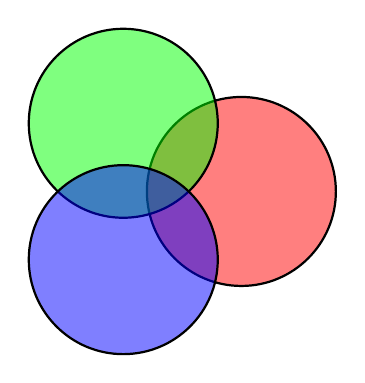
\begin{tikzpicture}[thick,fill opacity=0.5]
  \filldraw[fill=red]   (0:1cm)    circle (12mm);
  \filldraw[fill=green] (120:1cm)  circle (12mm);
  \filldraw[fill=blue]  (-120:1cm) circle (12mm);
\end{tikzpicture}
\end{codeexample}

\begin{codeexample}[]
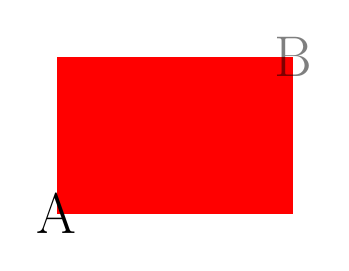
\begin{tikzpicture}
  \fill[red] (0,0) rectangle (3,2);

  \node                   at (0,0) {\huge A};
  \node[fill opacity=0.5] at (3,2) {\huge B};
\end{tikzpicture}
\end{codeexample}
\end{key}

\begin{key}{/tikz/text opacity=\meta{value}}
  Sets the opacity of text labels, overriding the |fill opacity| setting. 
\begin{codeexample}[]
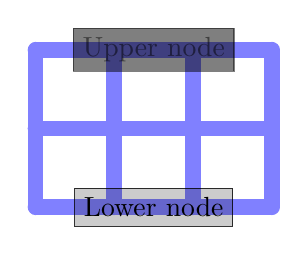
\begin{tikzpicture}[every node/.style={fill,draw}]
  \draw[line width=2mm,blue!50,cap=round] (0,0) grid (3,2);

  \node[opacity=0.5] at (1.5,2) {Upper node};
  \node[draw opacity=0.8,fill opacity=0.2,text opacity=1]
    at (1.5,0) {Lower node};
\end{tikzpicture}
\end{codeexample}
\end{key}


Note the following effect: If you setup a certain opacity for stroking
or filling and you stroke or fill the same area twice, the effect
accumulates:

\begin{codeexample}[]
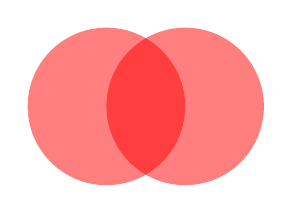
\begin{tikzpicture}[fill opacity=0.5]
  \fill[red] (0,0) circle (1);
  \fill[red] (1,0) circle (1);
\end{tikzpicture}
\end{codeexample}

Often, this is exactly what you intend, but not always. You can use
transparency groups, see the end of this section, to change this.



\subsection{Specifying a Fading}

For complicated graphics, uniform transparency settings are not always
sufficient. Suppose, for instance, that while you paint a picture, you
want the transparency to vary smoothly from completely opaque to
completely transparent. This is a ``shading-like'' transparency. For
such a form of transparency I will use the term \emph{fading} (as a
noun). They are also known as \emph{soft masks}, \emph{opacity masks},
\emph{masks}, or \emph{soft clips}.

How do we specify a fading? This is a bit of an art and you currently
need to use the basic layer, see Section~\ref{section-transparency} for
details. Under normal circumstance you will just use fadings that are
defined in the fading library. 

So, suppose a fading has been defined. It specifies for each pixel of
a certain area how transparent this pixel will be. The following
options are used to install such a fading in for the current scope or
path. The fading |fade down| used in the following examples gets more
and more transparent as we go from top to bottom.

\pgfdeclarefading{fade down}{%
  \tikzset{top color=pgftransparent!0,bottom color=pgftransparent!100}
  \pgfuseshading{axis}
}
\pgfdeclarefading{fade inside}{%
  \tikzset{inner color=pgftransparent!90,outer color=pgftransparent!30}
  \pgfuseshading{radial}
}

\begin{key}{/tikz/fade}
  This option tells \tikzname\ that the current path should be faded
  with the current fading. The current fading is set with the |fading|
  option, see below. Similarly to options like |draw| or |fill|,
  this option is reset for each path, so you have to add it to each
  path that should be faded.

  When the option is set, the fading is shifted and resized (in
  exactly the same way as a shading) so that is covers the current
  path. Then the path is drawn, but with the fading in force.
\begin{codeexample}[]
\begin{tikzpicture}[fading=fade down]
  % Checker board
  \fill [black!20] (0,0) rectangle (4,3);
  \path [pattern=checkerboard,pattern color=black!30] (0,0) rectangle (4,3);

  \fill [color=blue]      (0.5,1.5) rectangle +(1,1);
  \fill [color=blue,fade] (2.5,1.5) rectangle +(1,1);

  \fill [color=red,fade]  (1,0.75) ellipse (.75 and .5);
  \fill [color=red]       (3,0.75) ellipse (.75 and .5);
\end{tikzpicture}
\end{codeexample}

  \begin{key}{/tikz/fading=\meta{name}}
    Sets the fading to be used with the |fade| option to
    \meta{name}. The \meta{name} must previously have been defined
    (typically by a library). You can use this option with a scope or
    directly in a path to set the fading for the paths in the scope or
    for this single path. Setting this option inside a path also
    automatically sets the |fade| option (similarly to |shading| and
    |shade|).  
  \end{key}

  \begin{key}{/tikz/fading angle=\meta{degree} (initially 0)}
    Before the fading is used, it is rotate by \meta{degree}.

\begin{codeexample}[]
\begin{tikzpicture}[fading=fade down]
  % Checker board
  \fill [black!20] (0,0) rectangle (4,1.5);
  \path [pattern=checkerboard,pattern color=black!30] (0,0) rectangle (4,1.5);

  \fill [color=red,fade,fading angle=90]  (1,0.75) ellipse (.75 and .5);
  \fill [color=red,fade,fading angle=135] (3,0.75) ellipse (.75 and .5);
\end{tikzpicture}
\end{codeexample}
  \end{key}

  Note that you can ``fade just about anything.'' In particular, you
  can fade a shading.
  
\begin{codeexample}[]
\begin{tikzpicture}
  % Checker board
  \fill [black!20] (0,0) rectangle (4,4);
  \path [pattern=checkerboard,pattern color=black!30] (0,0) rectangle (4,4);

  \shade [ball color=blue,fading=fade down] (2,2) circle (1.8);
\end{tikzpicture}
\end{codeexample}

  The |fade inside| of the following example more transparent in the middle than on the
  outside.

\begin{codeexample}[]
\begin{tikzpicture}
  % Checker board
  \fill [black!20] (0,0) rectangle (4,4);
  \path [pattern=checkerboard,pattern color=black!30] (0,0) rectangle (4,4);

  \shade [ball color=blue]                     (3,3) circle (0.8);
  \shade [ball color=white,fading=fade inside] (1,1) circle (0.8);
  \shade [ball color=white,fading=fade inside] (2,2.5) circle (1.5);
\end{tikzpicture}
\end{codeexample}

\end{key}


% After having declared a fading, we can use it. As for shadings, there
% are two different commands for using fadings:

% \begin{command}{\pgfsetfading\marg{name}\marg{transformations}}
%   This command sets the graphic state parameter ``fading'' to a
%   previously defined fading \meta{name}. This graphic state works like
%   other graphic states, that is, is persists till the end of the
%   current scope or until a different transparency setting is chosen.

%   When the fading is installed, it will be centered on the origin with
%   its natural size. Anything outside the fading pictures's original
%   bounding box will be transparent and, thus, the fading effectively
%   clips against this bounding box.

%   The \meta{transformations} are applied to the fading before it is
%   used. They contain normal \pgfname\ transformation commands like
%   |\pgftransformshift|. You can also scale the fading using this
%   command. Note, however, that the transformation needs to be inverted
%   internally, which may result in inaccuracies and the following
%   graphics may be slightly distorted if you use a strong
%   \meta{transformation}.
% \begin{codeexample}[]
% \pgfdeclarefading{fading2}
% {\tikz \shade[left color=pgftransparent!0,
%               right color=pgftransparent!100] (0,0) rectangle (2,2);}    
% \begin{tikzpicture}
%   \fill [black!20] (0,0) rectangle (2,2);
%   \fill [black!30] (0,0) arc (180:0:1);
%   \pgfsetfading{fading2}{}
%   \fill [red] (0,0) rectangle (2,2);
% \end{tikzpicture}
% \end{codeexample}
% \begin{codeexample}[]
% \begin{tikzpicture}
%   \fill [black!20] (0,0) rectangle (2,2);
%   \fill [black!30] (0,0) arc (180:0:1);
%   \pgfsetfading{fading2}{\pgftransformshift{\pgfpoint{1cm}{1cm}}
%                          \pgftransformrotate{20}}
%   \fill [red] (0,0) rectangle (2,2);
% \end{tikzpicture}
% \end{codeexample}
% \end{command}

% \begin{command}{\pgfsetfadingforcurrentpath\marg{name}\marg{transformations}}
%   This command works like |\pgfsetfading|, but the fading is scaled
%   are transformed according to the following rules:
%   \begin{enumerate}
%   \item
%     It is assumed that the fading has a size of 100bp times 100bp.
%   \item
%     The fading is resized and shiften (using appropriate
%     transformations) such that the position
%     $(25\mathrm{bp},25\mathrm{bp})$ lies at the lower-left corner of
%     the current path and the position $(75\mathrm{bp},75\mathrm{bp})$
%     lies at the upper-right corner of the current path.
%   \end{enumerate}
%   Note that these rules are the same as the ones used in
%   |\pgfshadepath| for shadings. After these transformations, the
%   \meta{transformations} are executed (typically a rotation).
% \begin{codeexample}[]
% \pgfdeclarehorizontalshading{shading}{100bp}
% { color(0pt)=(transparent!0);    color(25bp)=(transparent!0);
%   color(75bp)=(transparent!100); color(100bp)=(transparent!100)}

% \pgfdeclarefading{fading}{\pgfuseshading{shading}}

% \begin{tikzpicture}
%   \fill [black!20] (0,0) rectangle (2,2);
%   \fill [black!30] (0,0) arc (180:0:1);

%   \pgfpathrectangle{\pgfpointorigin}{\pgfpoint{2cm}{1cm}}
%   \pgfsetfadingforcurrentpath{fading}{}
%   \pgfusepath{discard}
  
%   \fill [red] (0,0) rectangle (2,1);

%   \pgfpathrectangle{\pgfpoint{0cm}{1cm}}{\pgfpoint{2cm}{1cm}}
%   \pgfsetfadingforcurrentpath{fading}{\pgftransformrotate{90}}
%   \pgfusepath{discard}

%   \fill [red] (0,1) rectangle (2,2);
% \end{tikzpicture}
% \end{codeexample}

% \end{command}

\subsection{Transparency Groups}

% Consider the following cross and sign. They ``look wrong'' because we
% can see how they were constructed, while this is not really part of
% the desired effect. 

% \begin{codeexample}[]
% \begin{tikzpicture}
%   \pgfsetstrokeopacity{0.5}
%   \draw [line width=5mm] (0,0) -- (2,2);
%   \draw [line width=5mm] (2,0) -- (0,2);
% \end{tikzpicture}
% \end{codeexample}

% \begin{codeexample}[]
% \begin{tikzpicture}
%   \node at (0,0) [forbidden sign,line width=2ex,draw=red,fill=white] {Smoking};
%   \pgfsetstrokeopacity{0.5}
%   \pgfsetfillopacity{0.5}
%   \node at (2,0) [forbidden sign,line width=2ex,draw=red,fill=white] {Smoking};
% \end{tikzpicture}
% \end{codeexample}

% Transparency groups are used to render them correctly:

% \begin{codeexample}[]
% \begin{tikzpicture}
%   \pgfsetfillopacity{0.5}
%   \pgftransparencygroup
%     \draw [line width=5mm] (0,0) -- (2,2);
%     \draw [line width=5mm] (2,0) -- (0,2);
%   \endpgftransparencygroup
% \end{tikzpicture}
% \end{codeexample}

% \begin{codeexample}[]
% \begin{tikzpicture}
%   \node at (0,0) [forbidden sign,line width=2ex,draw=red,fill=white] {Smoking};
%   \pgfsetfillopacity{0.5}
%   \pgftransparencygroup
%     \node at (2,0) [forbidden sign,line width=2ex,draw=red,fill=white]
%       {Smoking};
%   \endpgftransparencygroup
% \end{tikzpicture}
% \end{codeexample}


% \begin{environment}{{pgftransparencygroup}}
%   This environment should only be used inside a |{pgfpicture}|. It has
%   the following effect:
%   \begin{enumerate}
%   \item The \meta{environment contents} is stroked/filled
%     ``ignoring any outside transparency.'' This means, all previous
%     transparency settings are ignored (you can still set transparency
%     inside the group, but never mind). This means that if in the
%     \meta{environment contents} you stroke a pixel three times in
%     black, it is just black. Stroking it white afterwards yields a
%     white pixel, and so on.
%   \item When the group is finished, it is painted as a whole. The 
%     \emph{fill} transparency settings are now applied to the resulting
%     picutre. For instance, the pixel that has been painted three times
%     in black and once in white is just white at the end, so this white
%     color will be blended with whatever is ``behind'' the group on the
%     page.
%   \end{enumerate}

%   Note that, depending on the driver, \pgfname\ may have to guess the
%   size of the contents of the transparency group (because such a group
%   is put in an XForm in \textsc{pdf} and a bounding box must be
%   supplied). \pgfname\ will use normally use the size of the picture's
%   bounding box at the end of the transparency group plus a safety
%   margin of 1cm. Under normal circumstances, this will work nicely
%   since the picture's bounding box contains everything
%   anyway. However, if you have switched off the picture size tracking
%   or if you are using canvas transformations, you may have to make
%   sure that the bounding box is big enough. The trick is to locallly
%   create a picture that is ``large enough'' and then insert this
%   picture into the main picture while ignoring the size. The following
%   example shows how this is done:

  
% \begin{codeexample}[]
% \begin{tikzpicture}
%   \draw [help lines] (0,0) grid (2,2);

%   % Stuff outside the picture, but still in a transparency group.
%   \node [left,overlay] at (0,1) {
%     \begin{tikzpicture}
%       \pgfsetfillopacity{0.5}
%       \pgftransparencygroup
%       \node at (2,0) [forbidden sign,line width=2ex,draw=red,fill=white]
%         {Smoking};
%       \endpgftransparencygroup
%     \end{tikzpicture}  
%   };
% \end{tikzpicture}
% \end{codeexample}


% \begin{plainenvironment}{{pgftransparencygroup}}
%   Plain \TeX\ version of the |{pgftransparencygroup}| environment.
% \end{plainenvironment}

% \begin{contextenvironment}{{pgftransparencygroup}}
%   This is the Con\TeX t version of the environment.
% \end{contextenvironment}

% \end{environment}


Consider the following cross and sign. They ``look wrong'' because we
can see how they were constructed, while this is not really part of
the desired effect. 

\begin{codeexample}[]

\begin{tikzpicture}
  \pgfsetstrokeopacity{0.5}
  \draw [line width=5mm] (0,0) -- (2,2);
  \draw [line width=5mm] (2,0) -- (0,2);
\end{tikzpicture}
\end{codeexample}

\begin{codeexample}[]
\begin{tikzpicture}
  \node at (0,0) [forbidden sign,line width=2ex,draw=red,fill=white] {Smoking};
  \pgfsetstrokeopacity{0.5}
  \pgfsetfillopacity{0.5}
  \node at (2,0) [forbidden sign,line width=2ex,draw=red,fill=white] {Smoking};
\end{tikzpicture}
\end{codeexample}

Transparency groups are used to render them correctly:

\begin{codeexample}[]

\begin{tikzpicture}
  \pgfsetfillopacity{0.5}
  \pgftransparencygroup
    \draw [line width=5mm] (0,0) -- (2,2);
    \draw [line width=5mm] (2,0) -- (0,2);
  \endpgftransparencygroup
\end{tikzpicture}
\end{codeexample}

\begin{codeexample}[]
\begin{tikzpicture}
  \node at (0,0) [forbidden sign,line width=2ex,draw=red,fill=white] {Smoking};
  \pgfsetfillopacity{0.5}
  \pgftransparencygroup
    \node at (2,0) [forbidden sign,line width=2ex,draw=red,fill=white]
      {Smoking};
  \endpgftransparencygroup
\end{tikzpicture}
\end{codeexample}




%%% Local Variables: 
%%% mode: latex
%%% TeX-master: "pgfmanual"
%%% End: 
